%
% 3-input-process-output.tex
%
%  LaTeX source file for section 3 Input-Process-Output for the Conceptual Clustering lab module of the TAILS project.
%

\section{Input-Process-Output}

\subsection{Input}
The input to this laboratory includes user-defined objects with various attributes and values. Let's say if we want to cluster different geometric figures, we may describe them  in multiple aspects, like shape, color or size. It's possible to have triangle, circle or rectangle. So here, \lq\lq{shape}\rq\rq, \lq\lq{color}\rq\rq and \lq\lq{size}\rq\rq are the attributes, and \lq\lq{triangle}\rq\rq, \lq\lq{circle}\rq\rq and \lq\lq{rectangle}\rq\rq are the attribute values for the attribute \lq\lq{shape}\rq\rq. The inputs for attributes and their values should be in the form of words only and it's case-insensitive. The input interface is shown in Figure \ref{Fig:intf1}. 
  \begin{figure}[h!]
     \centering
     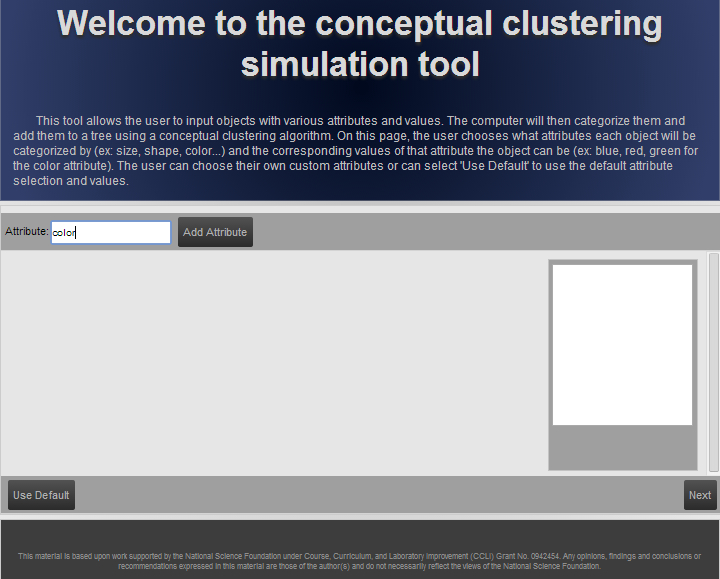
\includegraphics[width=300pt]{../images/interface1.jpg}
     \caption{The User Interface of Conceptual Clustering : Users can  input custom data either by the browser input or uploading from a file, or users can use the default setting}
     \label{Fig:intf1}   
     \end{figure}

If users want to input custom data, the tool allows for inputting data by the browser input or loading from a file. Using the browser input, users need to type in attribute names and their values accordingly. An attribute name should be typed in first in the attribute box and then click the \lq\lq{Add Attribute}\rq\rq button. The newly added attribute will be displayed under the input box. Moving the mouse on the attribute, the input box for attribute values will show up. Next, various values for the specific attribute can be typed in with the form of word only. An example is shown in Figure \ref{Fig:intf2}. 
 \begin{figure}[h!]
        \centering
        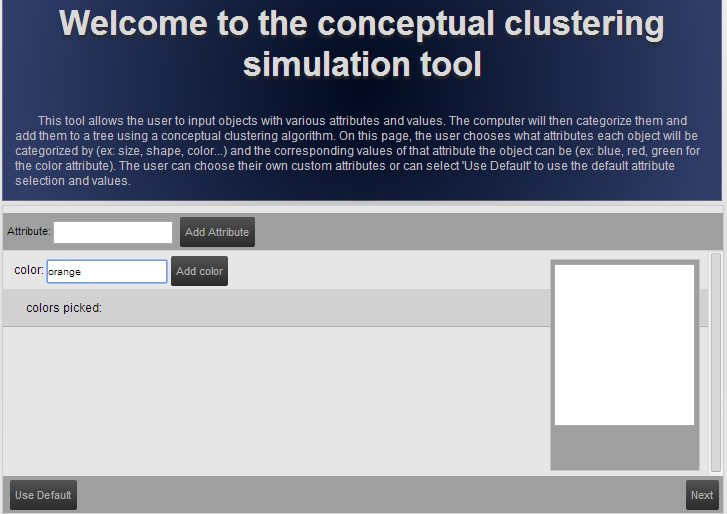
\includegraphics[width=300pt]{../images/interface2.jpg}
        \caption{Input custom data by the browser input}
        \label{Fig:intf2}
    \end{figure}

Users may also choose to load attributes and values from other documents by the box on the right. An example is shown in Figure \ref{Fig:intf2_loadfile}. These attributes are copied from a text file, which are  \lq\lq{color,size\#orange,blue,red\#large,small\#}\rq\rq. Clicking \lq\lq{Load Attributes}\rq\rq button, the custom data will be inputted. Whatever is loaded, the contents should follow the following rules:
\begin{enumerate}\renewcommand{\labelenumi}{(\theenumi)}\setlength{\itemsep}{0.05pt}
\item Attribute or values should be in the format of word only; 
\item Any attributes or values should be separated by a comma without a space;
\item Each line is separated by a pound sign \lq\lq{\#}\rq\rq;
\item The contents in first line will be identified as the attributes and the other lines will be recognized as the attribute values for each attribute defined in the first line;
\item An \lq\lq{Enter}\rq\rq at the end of each line makes no difference.
\end{enumerate}  
 \begin{figure}[h!]
       \centering
       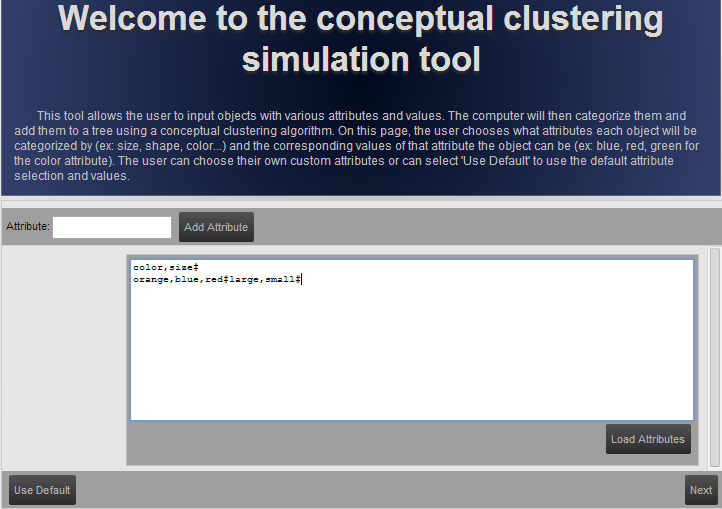
\includegraphics[width=300pt]{../images/interface2_loadfile.jpg}
       \caption{Input custom data by loading a file}
       \label{Fig:intf2_loadfile}
 \end{figure}  
 
Except for inputting custom attributes, users can click the \lq\lq{Use Default}\rq\rq button to use the default attribute selections and values. 	

\subsection {Process}
The simulation tool will display all the attributes and their values in the second interface and enable users to input different objects from the radio buttons. The tool will categorize the input objects and add them to a classification tree based on the COBWEB conceptual clustering algorithm. The second interface is shown in Figure\ref{Fig:intf3}. 
    
On the left, one or multiple objects can be added to generate the classification tree by selecting different attribute values and clicking \lq\lq{Add}\rq\rq or \lq\lq{Add Multiple}\rq\rq button. The dynamic graph of generating the classification tree will be displayed, showing how the clustering algorithm works. 
     
Moving the mouse on the node in the tree, the probabilistic concept label for this node will show up. The label includes the conditional probability for each attribute value given the current cluster, which corresponds to $P(A_i=V_{ij}\left|C_k\right.)$ and the percentage of the current cluster against the entire tree, which corresponds to $P(C_k)$ in the Category Utility function on Page 5. 

On the bottom of the visual window, every time a new object is added, there will be an explanation for what specific operation is carried out for the current step. Those operations are denoted as \lq\lq{Added node}\rq\rq, \lq\lq{Formed new subtree}\rq\rq, \lq\lq{Merged}\rq\rq and \lq\lq{Split}\rq\rq which correspond to the four COBWEB operations listed in Page 7.
    \begin{figure}[h!]
           \centering
           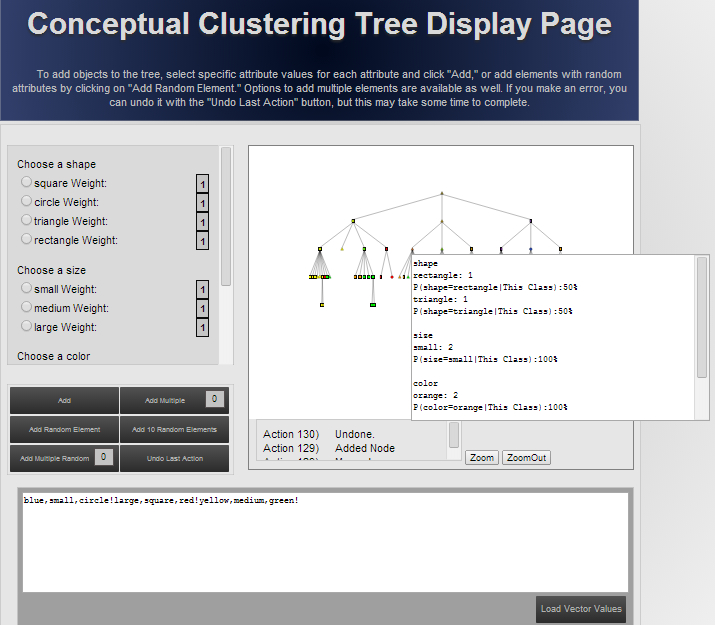
\includegraphics[width=300pt]{../images/interface3.jpg}
           \caption{The process of generating the clustering tree}
           \label{Fig:intf3}
     \end{figure}    
     
On the bottom of the tree display page, there is a input box allowing users to input objects by loading from other files. The format is the same as that for attribute, except that there should be an exclamation mark \lq\lq{!}\rq\rq separating the descriptions from one object to the next one. In the example shown in Figure \ref{Fig:intf3}, we copied \lq\lq{blue,small,circle!large,square,red!yellow,medium,green!}\rq\rq from a text file. By clicking \lq\lq{Load Vector Values}\rq\rq button, these objects will be added to the tree.

\subsection {Output}
The classification tree keeps spanning as long as more objects are added. The classification tree indicates the clusters for current input space. All the leaf nodes that share the same parent node is grouped into one cluster.
\subsection {Example}
 In this section, three experiments will be used to illustrate the effect of the input orders for the COBWEB algorithm. As we know, only one datum item is being considered at a time. The classification tree is sensitive to the input orders\cite{fisher1987knowledge}. The two operations merging and splitting are able to minimize the effect of the input orders but can not remove the effect.
 
 In order to observe the effect of the inputs orders, we carry out three experiments by using the same set of data in Table\ref{tab:inputseq}.
 \begin{table}[!ht]
 \ttabbox{\caption{Table of input data}}
 {
 \centering
 \begin{tabular}{l l l l l l l l}\hline
 \textbf{} & \textbf{shape} & \textbf{size} & \textbf{color}   & \textbf{} & \textbf{shape} & \textbf{size} & \textbf{color}\\\hline
 \textbf{1} & \textbf{square} & \textbf{large} & \textbf{blue}   & \textbf{6} & \textbf{circle} & \textbf{large} & \textbf{blue}\\
 \textbf{2} & \textbf{square} & \textbf{large} & \textbf{yellow} & \textbf{7} & \textbf{circle} & \textbf{large} & \textbf{yellow}\\
 \textbf{3} & \textbf{square} & \textbf{large} & \textbf{red}    & \textbf{8} & \textbf{circle} & \textbf{large} & \textbf{red}\\
 \textbf{4} & \textbf{square} & \textbf{large} & \textbf{orange} & \textbf{9} & \textbf{circle} & \textbf{large} & \textbf{orange}\\
 \textbf{5} & \textbf{square} & \textbf{large} & \textbf{green}  & \textbf{10} & \textbf{circle} & \textbf{large} & \textbf{green}\\
 \hline
 \end{tabular}
 \label{tab:inputseq}}
 \end{table}
 
 If we input the data with the sequence shown in the Table\ref{tab:inputseq}, the tree will be generated in the way shown in Figure\ref{Fig:inputseq1}. 
 \begin{figure}[h!]
            \centering
            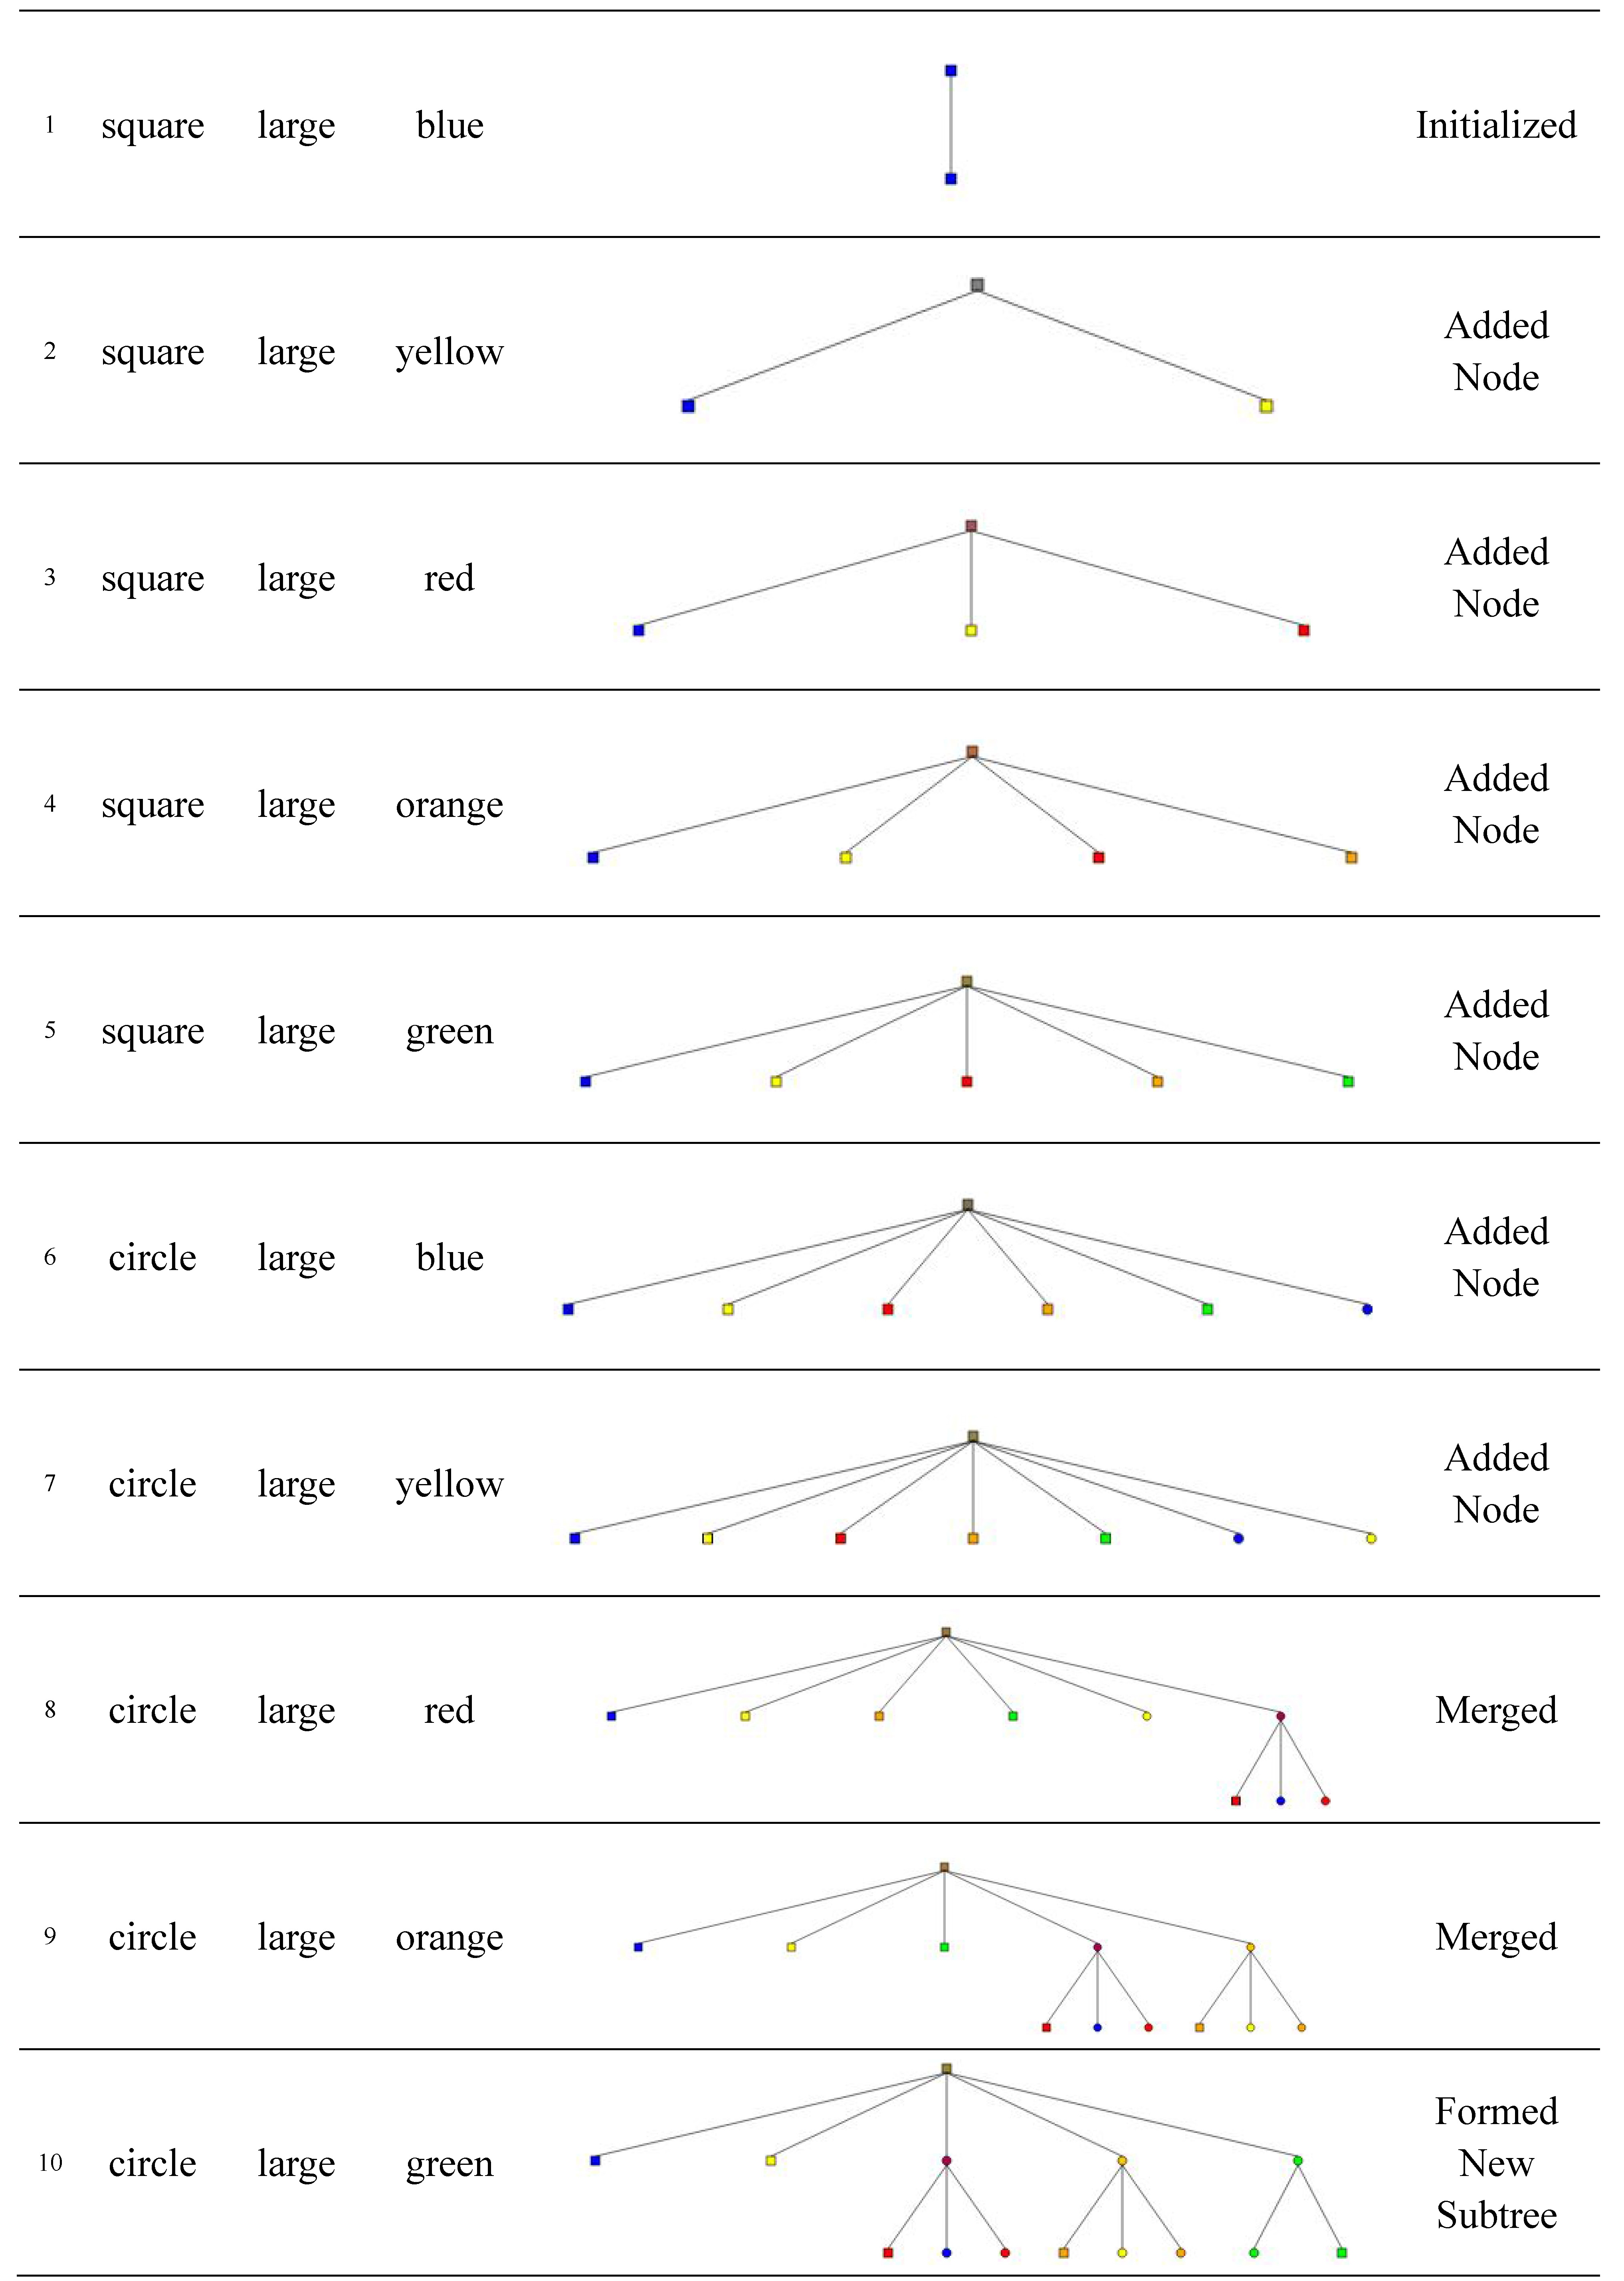
\includegraphics[width=420pt]{../images/inputseq1.jpg}
            \caption{The effect of input orders}
            \label{Fig:inputseq1}
 \end{figure}      

In the second experiment, we first input the blue square and blue circle and then followed by the yellow square and yellow circle and so on so forth till all the ten objects have been added. It's obvious that the tree is generated in a different way shown in the Figure\ref{Fig:inputseq2}.
\begin{figure}[h!]
            \centering
            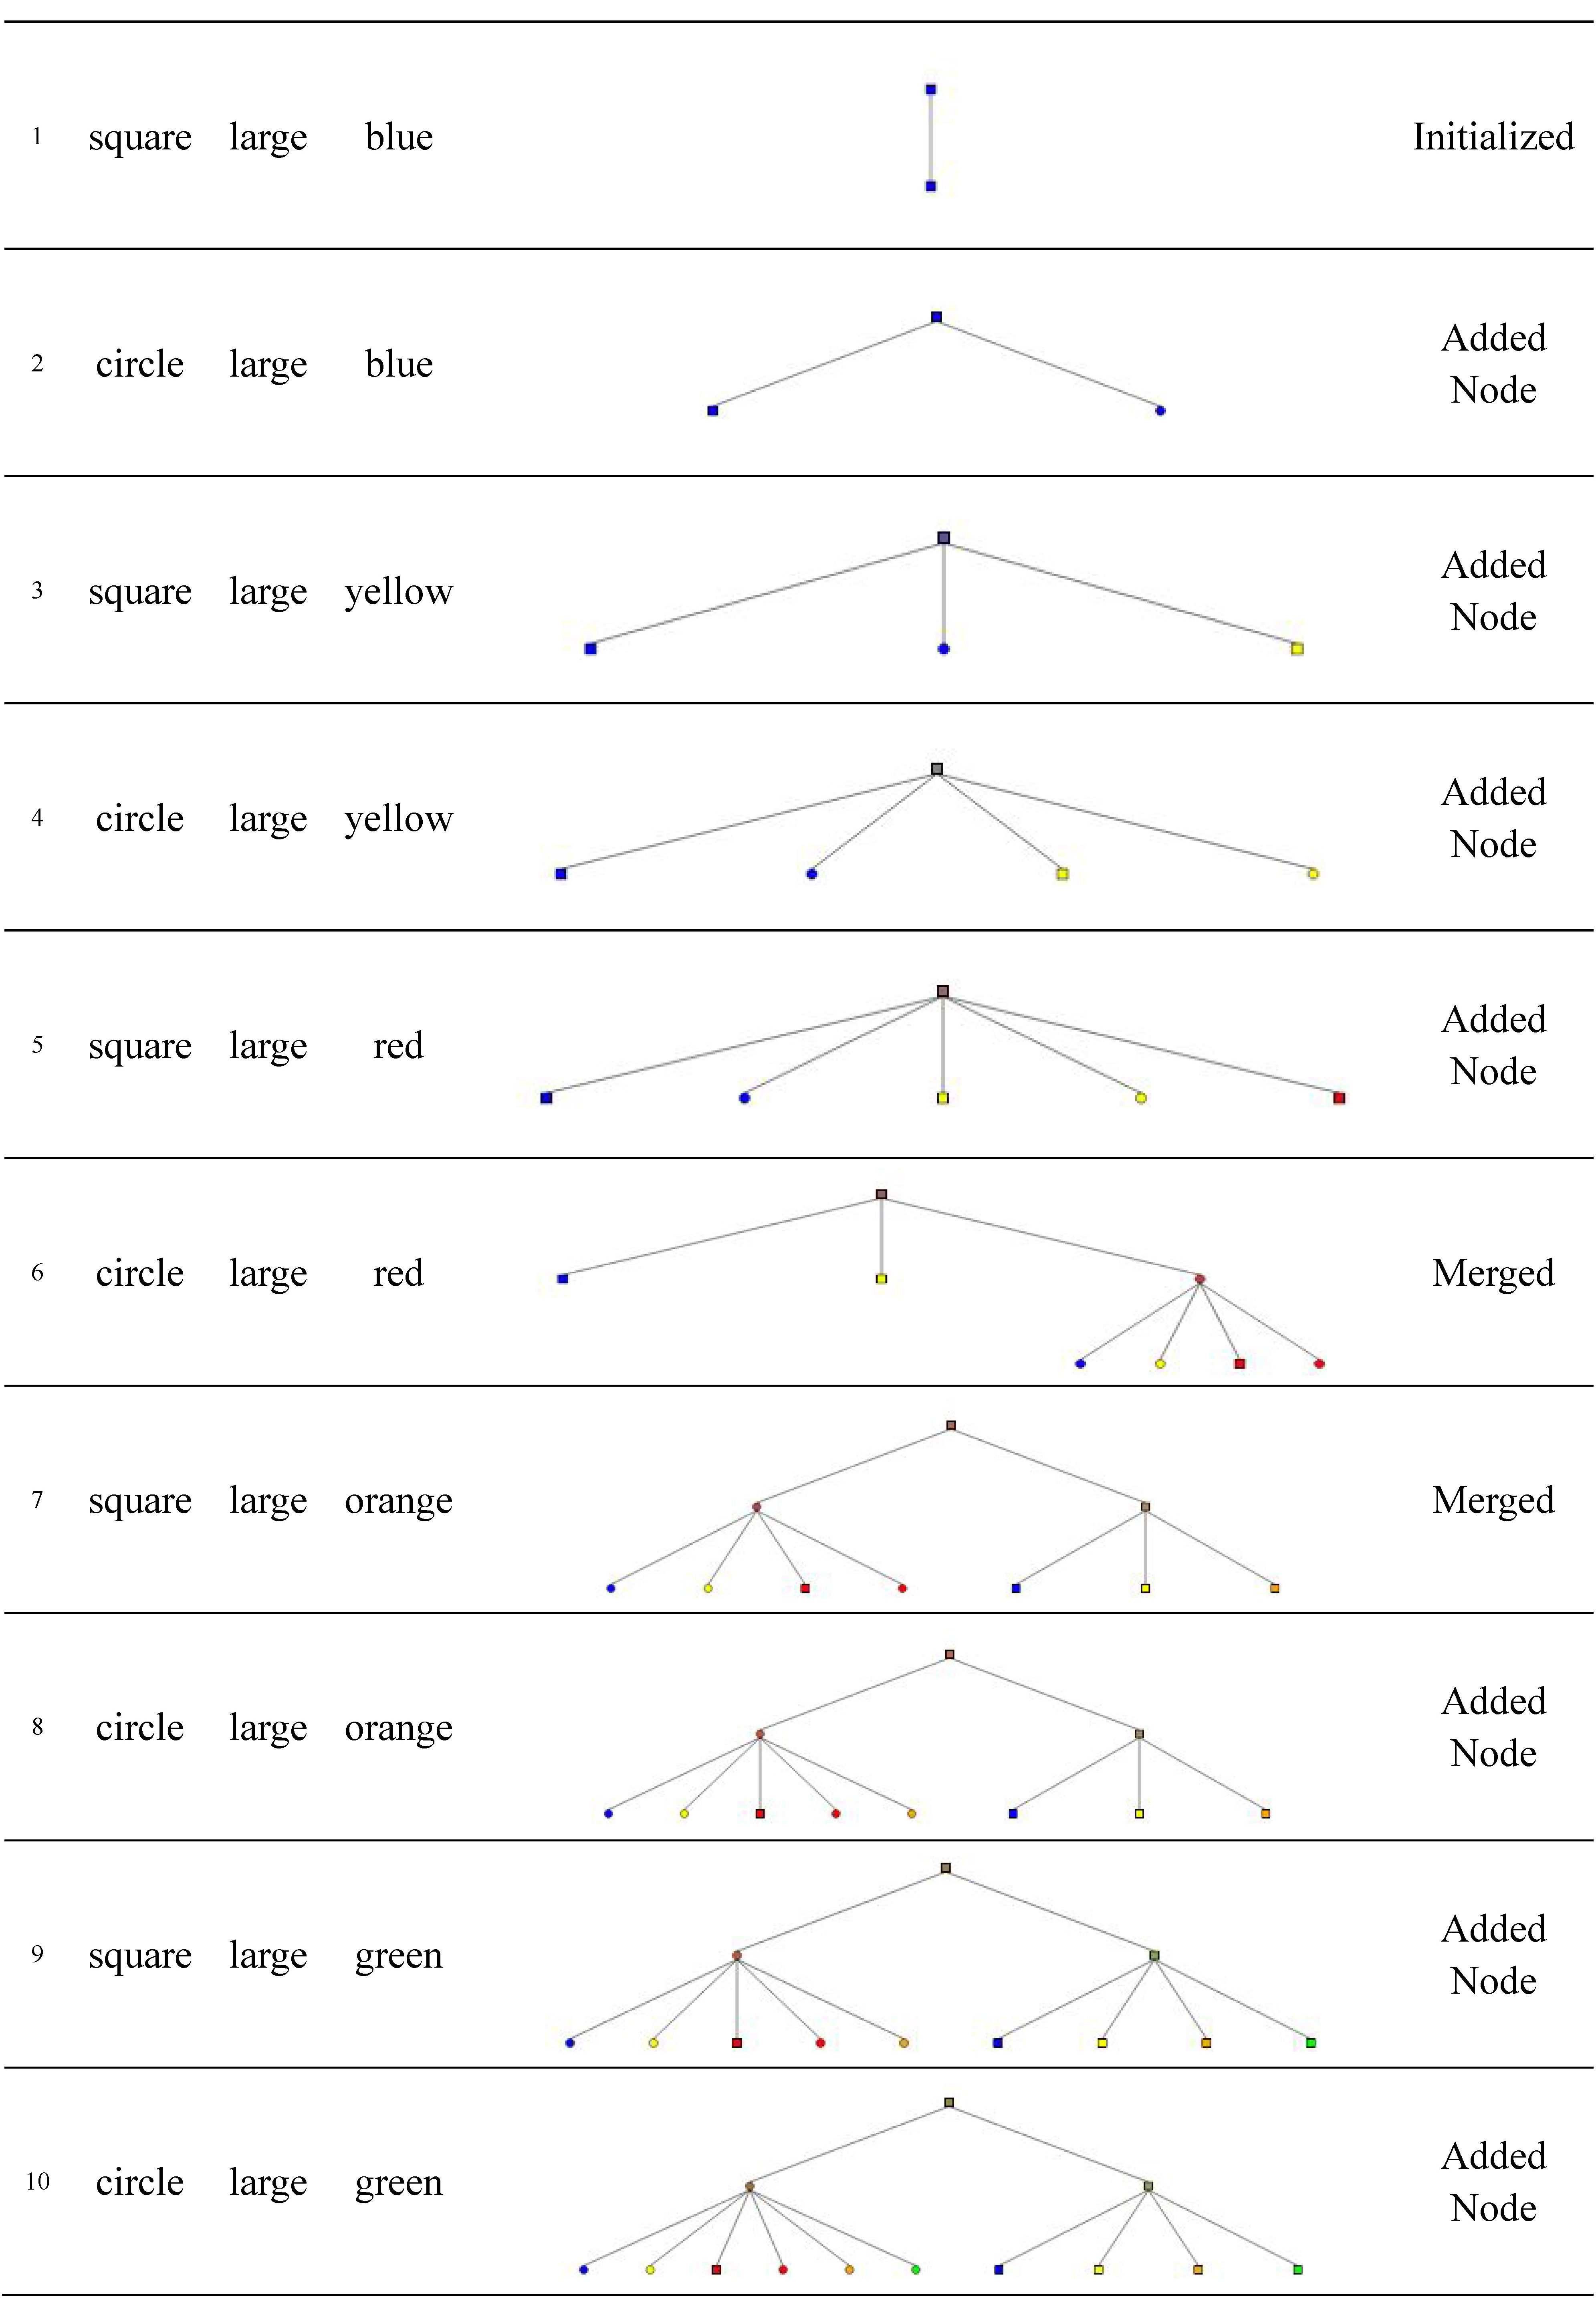
\includegraphics[width=420pt]{../images/inputseq2.jpg}
            \caption{The effect of input orders}
            \label{Fig:inputseq2}
 \end{figure}
 
 In the third experiment, we input the first three circles and then followed by the five squares and then the last two circles. The tree is generated in another way that is different from either of the previous two. The tree generated in the third experiment is shown in Figure\ref{Fig:inputseq3}.
 \begin{figure}[h!]
             \centering
             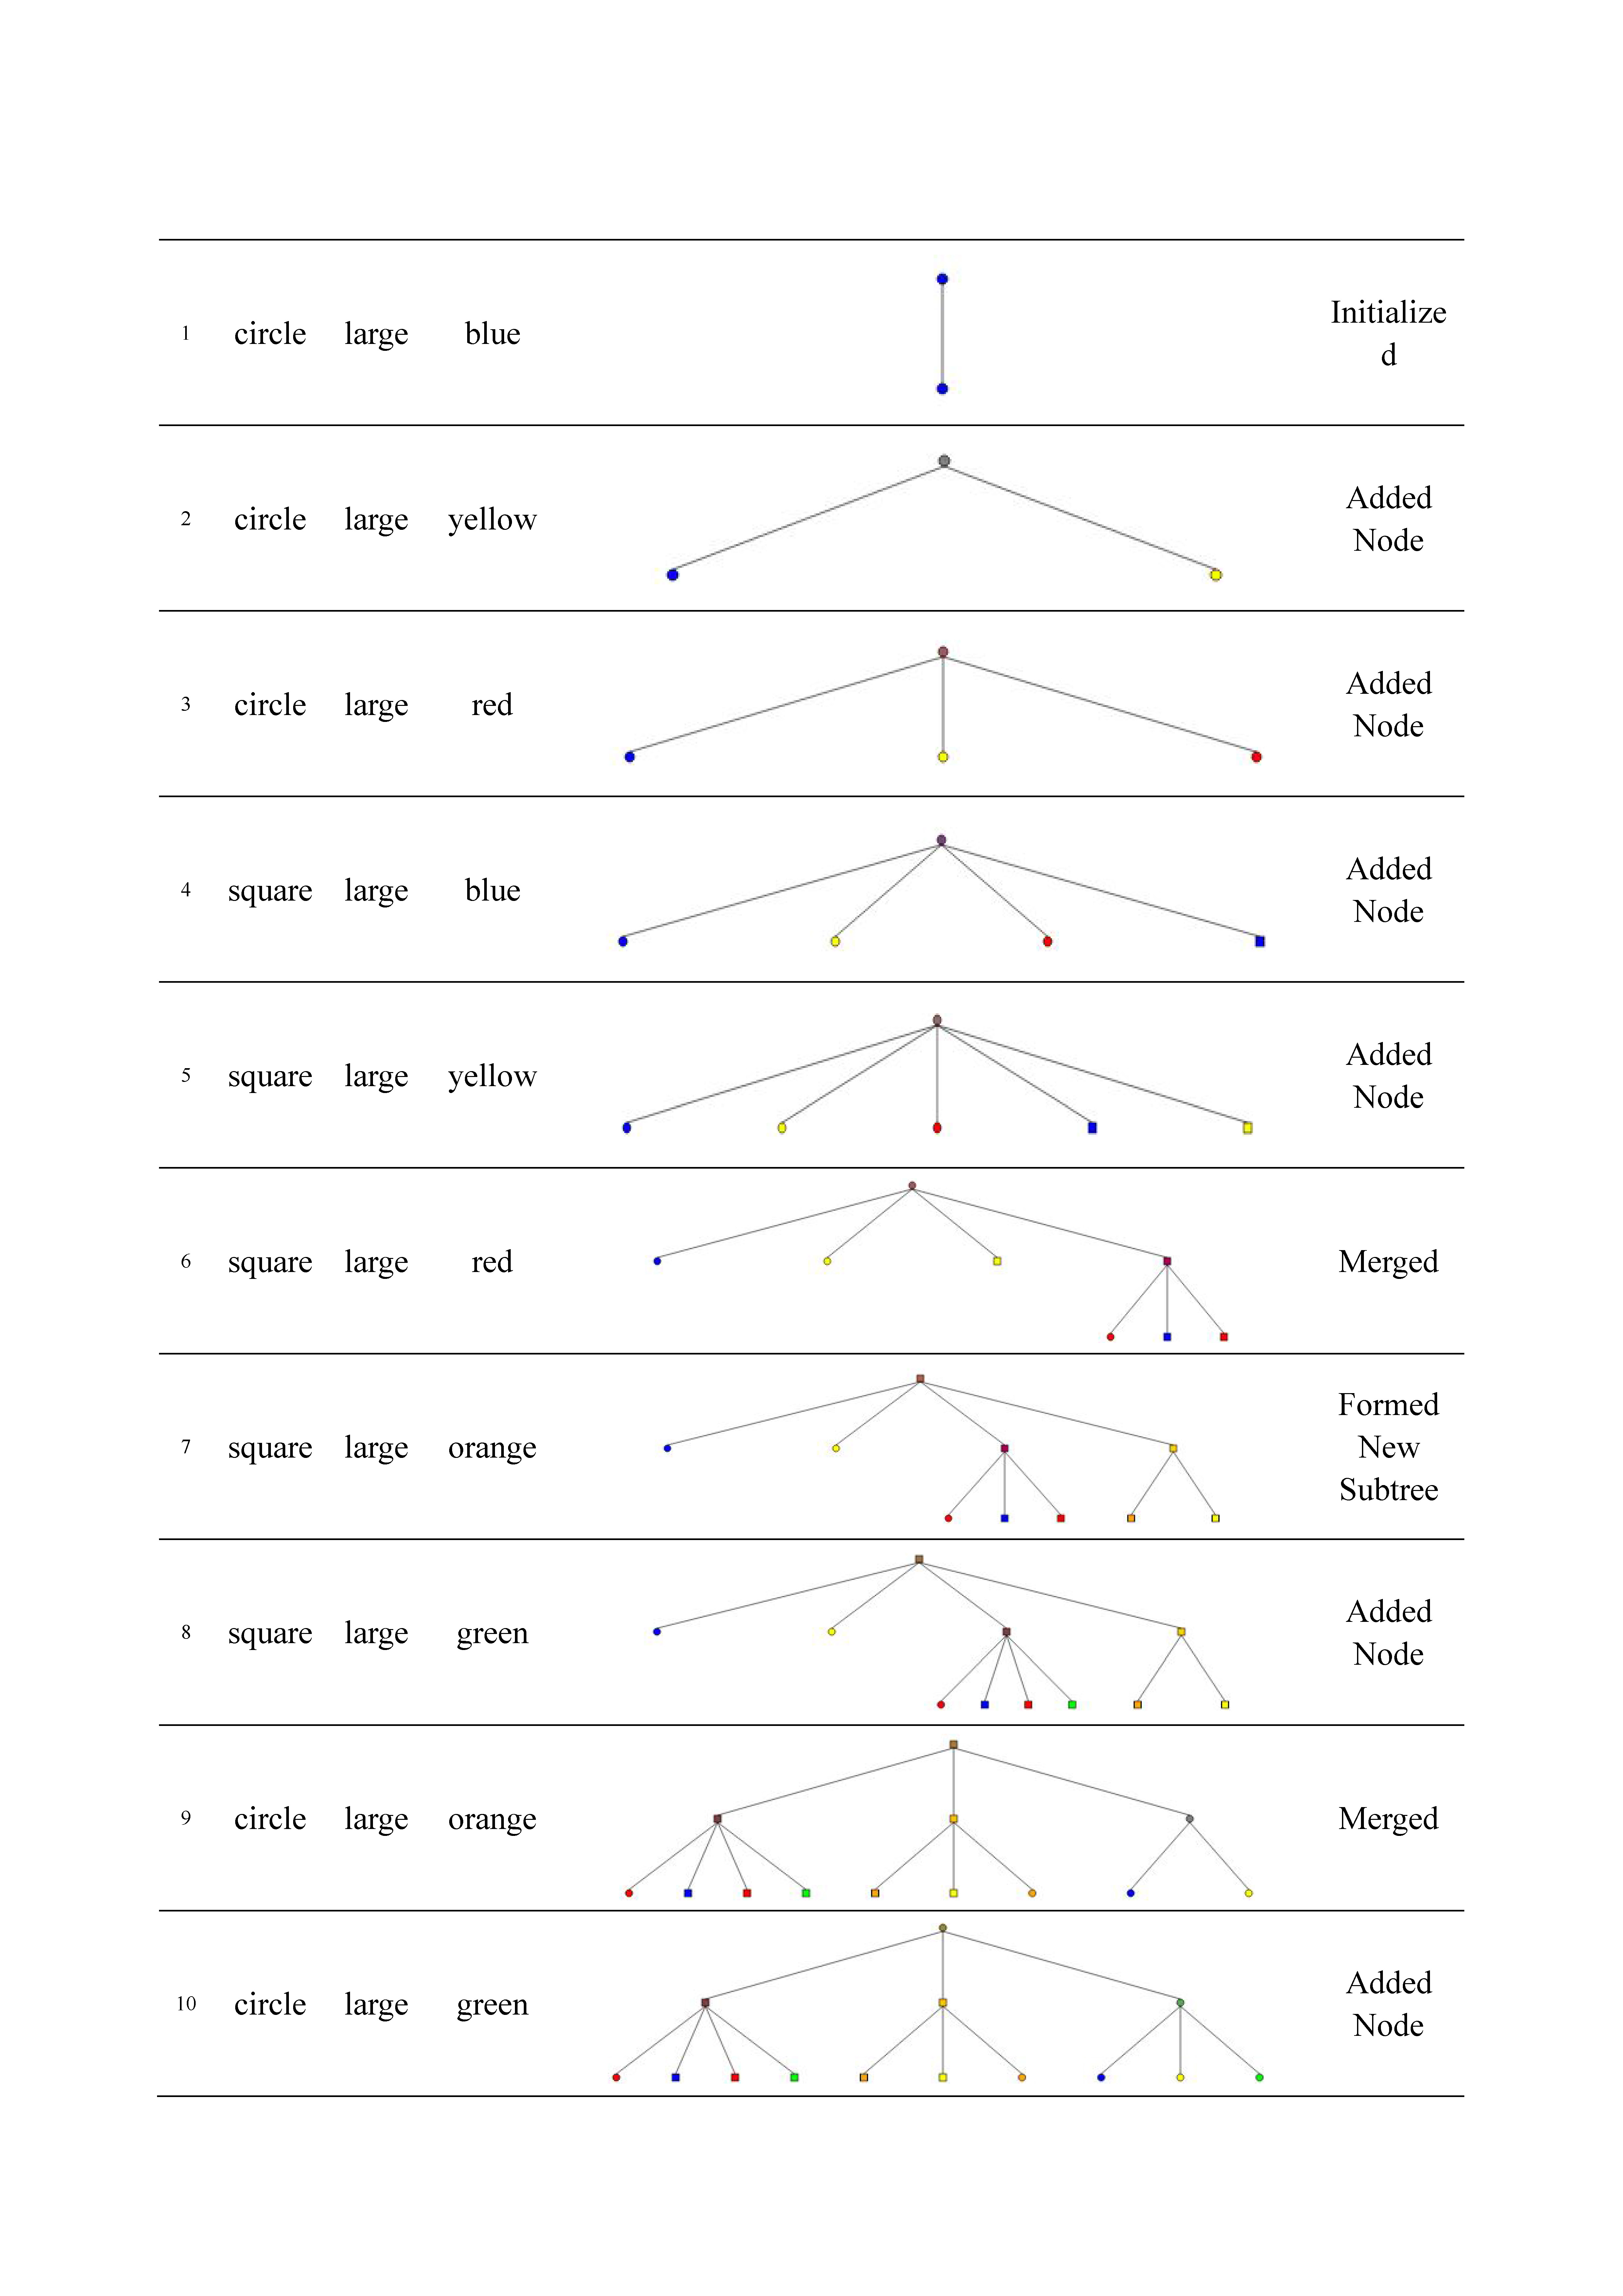
\includegraphics[width=420pt]{../images/inputseq3.jpg}
             \caption{The effect of input orders}
             \label{Fig:inputseq3}
  \end{figure}
 % %\newpage   
 %\includepdfmerge{../images/inputseq1.pdf}
 

    
    
    